\documentclass[a4paper]{article}
\usepackage{amssymb}
\usepackage{graphicx}
%\usepackage{hyperref}
\usepackage{microtype}
\usepackage{amsmath, amsthm, amssymb} 
\usepackage{caption}
\usepackage{subcaption}
\usepackage{subfig}
\usepackage{xargs}
\usepackage[pdftex,dvipsnames]{xcolor}  
\usepackage[colorinlistoftodos,prependcaption,textsize=tiny]{todonotes}
\newcommandx{\mytodo}[2][1=]{\todo[linecolor=red,backgroundcolor=red!25,bordercolor=red,#1]{#2}}
\usepackage{enumitem}
\usepackage{tabu}
\usepackage{array}

\title{H09M0A P\&D Embedded Systems and Multimedia \\ DSP}
\author{Seppe Iven - r0370830 \\ Koen Goetschalckx - r0375967}
\begin{document} 
\maketitle
\begin{center}Andras Boho, Yanxiang Huang
\end{center}
\section{Introduction}
This is a final report for the P\&D assignment on creating a speech codec. The goal of this project is to run an algorithm on a Digital Signal Processor that encodes, encrypts, decrypts and decodes speech in real-time. The encryption and decryption code is provided by another group. The codec implements subband filtering and adaptive quantization, with the goal of efficiently compressing a stereo audio signal.\\

First, a MATLAB implementation is written. A C implementation followed, and this is eventually ported onto a DSP and optimized. This paper follows the same order.
\section{Project description}
\subsection{Project overview}
\subsection{Main design specifications}
The following list contains the specifications that the design of the codec has to meet.

\begin{itemize}
\item It accepts stereo signals
\item The sampling frequency is 8 kHz
\item The bit rate is 24 kbit/s per channel codec, with good to very good speech quality
\item The implementation consists of a QMF tree-structured filterbank with polyphase implementation
\item An adaptive differential quantization scheme should be used for every subband signal
\item The filterbank of the codec consists of a minimum of 4 subbands
\item The total delay of the coder and decoder must not exceed a certain threshold: the entire one way communication delay (ADC, coding, encryption, decryption, decoding, DAC) should be less than 150 ms. This puts a maximum on the number of subbands, on the complexity of the filters and on the buffer size in the cryptography section. Note that the encryption and decryption functionality is provided by another group and is not a part of this assignment.
\item When running on the DSP, each stereo sample must be processed in less than 25000 cycles for real-time performance

\end{itemize}
\section{Splitting into subbands: QMF}
An input audio stream is split into subbands by using a Quadrature Mirror Filter bank.
A QMF filter bank consists of a low-pass and high-pass filter $H_0(z)$ and $H_1(z)$. These split the audio file into a low-frequency and a high-frequency part. Such filter bank is used to efficiently create a two-way filter bank. A recursive implementation is used to split an audio file into four subbands as shown by figure \ref{fig:qmfrecursive}.\\
\begin{figure}[hbt]
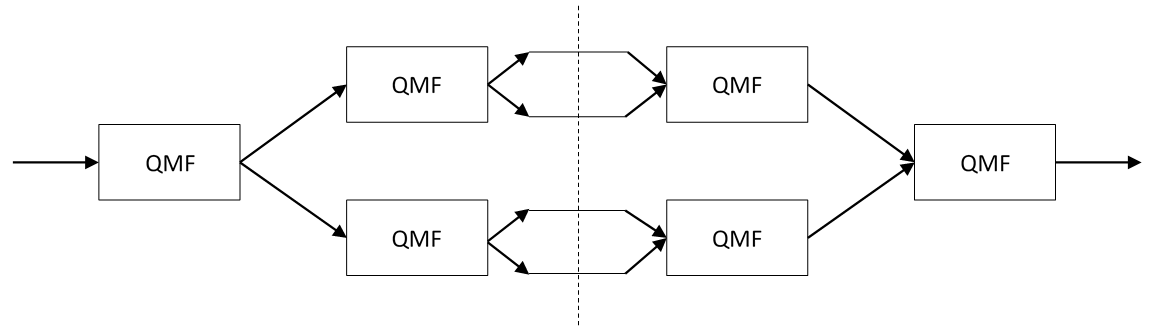
\includegraphics[width = \textwidth]{qmfrecursive}
\caption{four subbands QMF filter bank}
\label{fig:qmfrecursive}
\end{figure} \\
QMF filters have some special properties:
\begin{itemize}
\item if $H_0(z)$ is a QMF filter, then $H_1(z) = H_0(-z)$ has the frequency response of $H_0$ mirrored around $\pi/2$.
\item if $H_0(z)$ is a QMF filter, then analysis filters $H_0(z)$ and $H_1(z) = H_0(-z)$ and synthesis filters $F_0(z)=H_1(-z)=H_0(z)$ and $F_1(z)=-H_0(-z) = -H_1(z)$ form an alias-free filter bank.
\end{itemize}

The second property indicates that a complete alias-free QMF filter bank can be defined by $H_0(z)$ alone. For the filter to be linear phase, this $H_0$ should be chosen symmetrical. Also, the filter should have an even amount of taps to avoid distortion at half the Nyquist frequency. The first property indicates that if $H_0$ is a good low-pass filter, then $H_1$ is a good high-pass filter. \\

Given these properties and constraints, a simple polyphase implementation for a QMF filter bank can be designed, and is shown in figure \ref{fig:qmf}. The polyphase decomposition of $H_0(z)$ is:\\
\begin{center}
$H_0(z)$ = $E_0(z^2) + z^{-1} E_1(z^2)$ \\
\end{center}
From the first property, it follows that: \\
\begin{center}
$H_1(z)$ = $E_0(z^2) - z^{-1} E_1(z^2)$ \\
\end{center}
This leads to the efficient implementation of the filter bank shown in figure \ref{fig:qmf}.

\begin{figure}[hbt]
\includegraphics[width = \textwidth]{qmf}
\caption{Polyphase implementation of QMF filter bank}
\label{fig:qmf}
\end{figure}

For this project, both symmetric and asymmetric, where only one of the output bands of a QMF block are split further, structures were considered. Although for example 5 subbands created by always splitting the lower frequency band, may possibly have lead to better results, further use and study of these asymmetric structures were canceled as the teacher assistant said these were never considered previously and would lead to more complex C implementation. Thus, the final structure consists of QMF filter bank symmetrically splitting the signal into four subbands, as in figure \ref{fig:qmfrecursive}. Experiments show that four subbands can give good results in PESQ scores (discussed later). Eight or more subbands are thus not necessary but unwanted due to higher delay and computation complexity.

\section{Adaptive differential quantization}
After filtering into subbands, the data is now encoded with an adaptive differential quantization scheme. The quantizer can be seen in figure \ref{fig:quantization} and the dequantizer in figure \ref{fig:dequantization}. They contain the following signals:

\begin{itemize}
\item s(n) is the (serial) input signal
\item d(n) is the difference signal between the input signal and the prediction of the signal
\item z(n) is the quantized difference signal. This is also the output signal of the quantizer, hence the 'differential' in the name
\item d'(n) is the difference signal after quantization and dequantization. It thus resembles d(n) but is not exactly the same value
\item s'(n) is the sum of d'(n) and the prediction. It thus resembles s(n) but is not exactly the same value
\item s*(n) is the prediction of the next input signal 
\end{itemize}

The step size is adaptive and based on the last values of d'(n) and a parameter $\phi$. The amount of values that influence the step size, is determined by a parameter 'buffer\_length'. Step size is calculated as follows:
\begin{equation*}
stepsize = round\_to\_zero(\phi*mean(abs(D'(n))))
\end{equation*}
Herein D'(n) contains the last buffer\_length values of d'(n). The mean should be zero, thus this equals the first central moment. This is chosen instead of the variance for easy of calculation. \\
The reason of the use of d'(n) instead of d(n) is because the dequantizer only knows d'(n) and not d(n). For the same reason, the prediction is based on s'(n) and not in s(n). The prediction is a simple first order prediction, defined by the previous approximation of the signal s'(n) and a parameter $\mu$:
\begin{equation*}
s^*(n) = \mu*s'(n-1)
\end{equation*}
The dequantizer can reconstruct s'(n) based on the z(n) it receives. The system is thus lossy, since it cannot reconstruct the exact signal s(n). The benefit of this system is that the only transmitted signal is z(n), whose range is normally smaller than the range of s(n). Thus less bits are needed for encoding and transmitting z(n) than for s(n) and lossy compression is realized.
\begin{figure}[hbt]
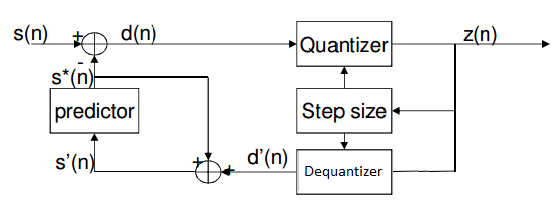
\includegraphics[width = \textwidth]{Quantization.png}
\caption{The Adaptive Differential Quantization scheme}
\label{fig:quantization}
\end{figure}
\begin{figure}[hbt]
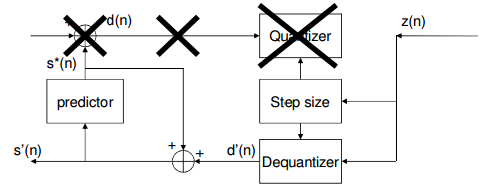
\includegraphics[width = \textwidth]{Dequantization.png}
\caption{The Adaptive Differential Dequantization scheme}
\label{fig:dequantization}
\end{figure}

Both the quantizer and dequantizer are initialized with the initial prediction $s^*(0) = 0$ and the initial $stepsize(0) = 1$.
\section{MATLAB implementation}
This section gives a brief explanation of the used MATLAB files and their functionality.

\subsection{generate\_some\_params.m and test\_some\_params.m}
These script can be run to generate parameters used to call run. After generating the parameters, test\_some\_params also calls run on 8 audio files and calculates the average PESQ and SNR scores.

\subsection{run.m}
This is the main function used to divide an audio file into subbands, quantize and dequantize those subbands, and synthesize them again to create an audio signal that closely resembles the original signal. Accepted audio files are .wav-files that are stereo or pairwise mono. The input audio file that should be used is passed as an argument.\\

The input is scaled to a 16-bit signed integer. The input is then split into subbands by calling analysis.m. These subbands are first quantized by calling quantize.m. The result that is now obtained, is the signal that would be saved or transmitted in real use. Next, the function dequantizes the result by calling dequantize.m. Finally, calling synthesis.m recombines the subbands and the PESQ score for the reconstructed audio file is calculated. For this calculation, only one channel is considered, because in most of the test files the two channels are the same (effectively mono). Even when this is not the case, a noticeable increase of score in one channel should lead to a similar increase in the other for real life signals.

\subsection{analysis.m}
This MATLAB function splits the stereo (or pairwise mono) channels into separate channels, and splits them into subbands by calling get\_subbands.m.

\subsection{get\_subbands.m}
This function recursively splits an audio signal into its subbands. It does this by applying polyphase QMF filters, as explained earlier in this paper. These filters are generated with a function that was given as part of the assignment and characterized defined by its parameters.\\

Convolutions are used to apply the filters. Since this is a sum of products, the output values exceed the 16-bit range. The output must thus be downscaled again. This downscaling is done by division of a power of two, so it is easily implementable as a bit shift. The exponent of two can be chosen, as it is a parameter of this function. It should however be chosen with respect to the filter length: longer filters add more numbers, creating a larger result and thus the need for more downscaling. The choice of exponent gives rise to a trade-off between clipping and quantization noise. An exponent that is too small leads to the former, while a too large exponent leads to relatively larger quantization noise.

\subsection{quantize.m}
This function uses the earlier mentioned adaptive differential quantization method to compress an input signal. A parameter determines the maximum output and thereby the amount of bits needed. Larger values are clipped. This should be avoided by changing the other parameters. For analysis purposes, the function keeps track of the number of times the clippings happened. Input parameters $\phi$ and $\mu$ must be scaled to signed 16-bit integers.

\subsection{dequantize.m}
This function is the inverse of quantize.m: it takes the output of the adaptive differential quantisation function and constructs s'(n), which approximate the original input signal s(n). Parameters $\phi$ and $\mu$ and 'buffer\_length' should be the same as those used for encoding with quantize.m.


\subsection{synthesis.m}
This function is the inverse of get\_subbands.m: its inputs are the separate subbands and it combines (synthesizes) them into one signal. The filters used for this are the same QMF filters used for analysis, as explained earlier in the text. As in analysis.m, scaling is done to refit the values into the 16-bit range.

\section{Parameter values and their PESQ and SNR scores}
\subsection{Proposed values of controllable parameters}
This section handles all of the parameters that define the implementation of the speech codec.\\

The QMF filters generated with the given function QMF\_design.m are characterized by the following parameters:

\begin{itemize}
\item The sampling frequency, which is mandatory 8 kHz
\item The total transition width of the prototype filter. This is default at a tenth of the sampling rate, and thus we have left it at 800
\item The minimum stopband attenuation of the prototype filter, which we changed to 300dB for the filter that further splits the high-frequency channel and to 50dB for the other two filters
\item The frequency step for finding the optimal cut-off frequency, which we have left at the default value of 10
\item The maximum number of iterations, which we have at 600
\item The filter lengths, which we have at 64 for the filter at the first depth and 32 for the filters at the second depth. We have chosen these lengths as a compromise between filter quality and implementation delay
\
\end{itemize}

The encoding parameters $\mu$, $\phi$, buffer\_length and the number of bits per sample can be different for each subband. The values for all these parameters are listed in table \ref{tab:parametervalues}. Table \ref{tab:scalingparameters} shows the amount of scaling used after the convolutions in each QMF filter.

\begin{table}[h]
\centering
\begin{tabular}{l|cccc} 
band frequency & lowest & low & high & highest \\ 
\hline 
\#bits & 5 & 4 & 3 & 0 \\ 
$\mu$ & 19660 & 328 & 31129 & / \\  
$\phi$ & 5144 & 16384 & 29490 & / \\  
buffer\_length & 10 & 10 & 10 & / \\  
\hline 
\end{tabular}
\caption{Current optimal values of encoding parameters}
\label{tab:parametervalues}
\end{table}
\begin{table}[h]
\centering
\begin{tabular}{c|ccc}
\multicolumn{4}{c}{Analysis filter bank}\\
\hline
\hline
scalings & lower frequencies & • &  higher frequencies \\ 
\hline 
depth 1 &  • & 15 & •  \\ 
depth 2 &  15 & • & 15  \\ 
\hline 
\multicolumn{4}{c}{}\\
\multicolumn{4}{c}{Synthesis filter bank}\\
\hline 
\hline
scalings & lower frequencies & • &  higher frequencies \\ 
\hline 
depth 1 &  • & 13 & •  \\ 
depth 2 &  15 & • & 15  \\ 
\hline 
\end{tabular} 
\caption{Current scaling parameters (\#bits to shift)}
\label{tab:scalingparameters}
\end{table}
Lower subbands have more bits per sample, since they are more important to the human hearing. Notice that the highest frequencies are simply thrown away. Finding the other values started by chosing the values for the scaling, because these give very high differences in PESQ scores. One division by 2 (one bitshift) too many results in a lower amplitude of the signal, one too few leads to clipping and thus distortion. Next the buffer\_lengths were changed. The length for the lowest frequency made a large difference. The others did not have much influence and were thus set to the same value for easy implementation. From this point on $\mu$, $\phi$ and buffer\_length values were changed one by one, always selecting a value that increased the average PESQ score. It is comparable to a greedy optimizing algorithm. This way lead to mentioned values.\\

\subsection{SNR \& PESQ score}
The perceptual metric PESQ is used to grade the quality of the codec. It was decided to use PESQ instead of SNR since it takes features of the human hearing into account (such as masking). This is why the optimal values are chosen on basis of PESQ scores, and SNR is mainly ignored.\\

\begin{table}[bth]
\begin{center}
\begin{tabular}{ l|ll }
  File name & PESQ score & Segmental SNR \\
  \hline
  belasting & 3.41 & 17.44\\
  bir & 3.51 & 17.59\\
  f116 & 3.22 & 14.11 \\
  f216 & 3.00 & 16.98\\
  m116 & 3.29 & 13.26\\
  m216 & 3.38 & 12.31\\
  words\_f & 3.51 & 18.61\\
  words\_m & 3.54 & 16.12\\
  \hline
\end{tabular}
  \caption{PESQ and segmental SNR scores for different audio files}
\label{tab:pesqscores}
\end{center}
\end{table}
The parameters are optimized by maximizing the average PESQ score of the files in table \ref{tab:pesqscores}. This is preferred to a single file, since it contains more variation as training data. All files were equally weighted in the average. All audio streams were delivered at 16kHz sampling rate, but the system is designed for 8kHz. Using Audacity, an anti-aliasing filter with 70dB attenuation for frequencies above 4kHz was applied to these audio files, before downsampling them to 8kHz. The values in table \ref{tab:pesqscores} are obtained using run.m with these downsampled versions.

\subsection{Inherent delay of the implementation}
The filters used in the QMF filter bank lead to a delay. For each depth in the filterbank, the delay is given by $delay_i = (n_i-1) / sample\_rate_i$ with $i$ the depth, $n_i$ the amount of filter taps at this depth and $sample\_rate_i$ the sample rate at this depth, which is equal to the original sample rate divided by $2^{i-1}$. With filters of 64 and 32 taps, the delay becomes:
\begin{equation*}
delay = \frac{(64-1)}{8000 Hz} + \frac{(32-1)}{4000 Hz} = 15.625 ms.
\end{equation*}

\section{Evaluation of MATLAB code}
The MATLAB code is designed to be very flexible, with easy to change, grouped parameters. All MATLAB functions work with fixed point values. This simulates the workings of a DSP. All performance results should therefore not change when the system is run on a DSP. The achieved PESQ scores (3.00 to 3.54) were shown and indicate decent performance. The optimal values of the parameters were found by searching for the highest PESQ score by changing the parameters one by one. Finally, the inherent delay of the implementation was briefly discussed and calculated to be less than $16ms$. This leaves $134ms$ for the encryption and decryption, processing and other kinds of buffering.\\


While translating the MATLAB code to C (see below), it became clear that although the MATLAB code can use asymetric filter banks, it is not implemented properly: a path with less filters or filters of smaller order is not extra delayed to have the same delay as the longer path. This error is not fixed, since we decided not to use an asymmetric structure anyway.

\section{C implementation on a PC}
Given the MATLAB model for the codec, the next task is to translate this code into an efficient implementation in C. This can later on be ported onto a Digital Signal Processor.
\subsection{Differences between the MATLAB and C implementation}\label{sec:differences}
\subsubsection{Flexibility}
The MATLAB code offers more flexibility than the C code. In MATLAB, even the structure of the analysis and synthesis filter banks (e.g. the amount of subbands) can be derived from given parameters. In C however, this structure is fixed in the code.\\

The parameters are also more cumbersome to change in the C code. In MATLAB, they are nicely grouped in \texttt{generate\_some\_params.m} or \texttt{test\_some\_ params.m} and given as arguments to the main routine (\texttt{run.m}). In C however, most of them are hard coded. The parameters for \texttt{quantize} and \texttt{dequantize} can relatively easily be found and changed at the the beginning of \texttt{main.c}. The parameters for the highest frequency subband cannot be changed at all: it is hard coded that this band is completely removed. This subband is consequently not quantized nor dequantized. Changing this would require adjustments to \texttt{mainencode}, \texttt{maindecode}, \texttt{compress30samples} and \texttt{decompress30samples}. Any other change in the number of bits assigned to the subbands would require complex changes to only the latter two.\\

All the parameters of the filterbanks are also difficult to change. In MATLAB, the filters are generated based on given parameters while in C, the filters themselves must be entered. This removes the flexibility of easily changing their length or stopband attenuation. Also the amount of scaling to be done after applying the filters, is hardcoded in the C functions \texttt{analysis} and \texttt{synthesis} and can therefore not be changed very quickly.

\subsubsection{Rounding and scaling}\label{sec:rounding}
Although the MATLAB implementation was designed to mimic C like integer operations, some false assumptions were made. Table \ref{tbl:roundingassumptions} lists these, as well as their correction and solution. The purpose of the solutions is always to make the C implementation consistent with the MATLAB implementation. The second solution might make the code a little slower, but because it is not in the critical inner loop of \texttt{convolve} (see \ref{sec:processing}), it does not make an important difference.\\

Apart from the changes mentioned in table \ref{tbl:roundingassumptions}, another change was made in MATLAB: the values that are loaded from the .wav-file are multiplied by $2^{15}$ instead of scaled to use the full integer range. This is not the same when the values in the .wav-file do not occupy their full available range. This change is made because the maximum value must be known in order to scale the values to the full available range. This information is not known in a real-time application, and can thus not be used.
\begin{table}[htb]
\centering
\makebox[\linewidth][c]{
\tabulinesep=1.2mm
\begin{tabu}{p{3.0cm}>{\centering\arraybackslash}p{1.7cm}p{3.5cm}>{\centering\arraybackslash}p{1.7cm}p{4cm}}
False assumption & Examples & Correction & Examples & Solution \\
\hline
\hline
MATLAB rounds integer divisions towards zero (like C) & 
	10/6 = 1 \quad (-9)/2 = -4 &
	 MATLAB rounds towards nearest integer (halves away from zero) &
	  10/6 = 2 \quad(-9)/2 = -5 &
	  MATLAB division \texttt{a/b} changed to \texttt{int16(fix( double(a)/double(b)))}.\\
\hline
C rounds the result of a division by shift towards zero &
	-9\texttt{>>}1 = -4 \quad 9\texttt{>>}1 = 4 &
	C does floor on the result&
	-9\texttt{>>}1 = -5 \quad 9\texttt{>>}1 = 4 &
	a\texttt{>>}b was replaced by \texttt{a/(1\texttt{<<}b)} in the C code.

\end{tabu}
}
\caption{False assumptions about rounding mechanisms, with their corrections and solutions}
\label{tbl:roundingassumptions}
\end{table}

\subsubsection{Execution order}
The MATLAB implementation is just for quality testing, for which the complete input signal can be known at starting time. Therefore, a whole .wav-file can be and is loaded at the start. Each intermediate signal, e.g. the result of a convolution, is calculated over the full length of the signal at once. Only after the full signal is calculated, it is passed to further calculations. This simplifies the code. The C code however, targets a real time-application. The complete input signal is thus not known beforehand. Waiting until the complete signal is received is impossible, because the delay would be unacceptable and the length of the input is not bounded. Therefore, the C code works buffer per buffer. It reads a specified amount of values and saves them in a buffer. On this buffer, all calculations are performed and the final output is received immediately without waiting for the rest of the signal. When the final output for the current buffer is calculated, a new buffer is read. The delay is thus no more than the time it takes to fill the buffer added to the intrinsic delay of the filterbank. The time needed to calculate the output of an input buffer should be negligible. \\

The analysis and synthesis functions do not only require the samples of the current buffer, but also older samples and older intermediate values to do the convolutions. The quantization and dequantization functions require previous samples to calculate the moving average. To do this, both functions use a structure containing previous samples.

\subsection{Compression: preparation to communicate with crypto part}\label{sec:communication}
The quantization function outputs shorts. However, these shorts contain only a small amount of effective bits, because the actual range of the values is limited. The samples of every subband will be quantized to 5, 4, 3 or 0 effective bits per sample, from lowest to highest frequency subband respectively. The function \texttt{compress30samples} takes 30 samples as shorts, 5 from each except the highest subband of both channels, and performs bitwise operations on them to take only their effective bits and to put them in 15 bytes. These 15 bytes then contain all the necessary information for dequantizing the samples and feeding them to the synthesis filter bank, without any unnecessary bits. These bytes can easily be passed to the encryption algorithm. Function \texttt{decompress30samples} implements the inverse of \texttt{compress30samples} and can be used on 15 decrypted bytes to recalculate the original 30 samples.	


\subsection{Performance enhancements made before porting}\label{sec:performance}
\subsubsection{Memory}
To avoid wasting memory, all these functions work in place, meaning they write their output on the same place as they read their input:
\begin{itemize}[noitemsep]
\item \texttt{compress30samples}
\item \texttt{combineWithoutDelay}
\item \texttt{convolve}
\item \texttt{combine}
\end{itemize}
Writing the output in place removes the necessity of reserving memory for both the input and the output. With our implementation, this comes at a cost of more complex indexing, as reading or writing `after the end' of the array must equal reading or writing at the beginning of the array. This can easily but inefficiently be implemented by doing a modulo operation on the index. A more efficient implementation is used in the \texttt{convolve} function, as the following subsection clarifies.
\subsubsection{Execution time}\label{sec:processing}
After finishing a first complete and fully functioning version of the code, Visual Studio's\footnote{Microsoft Visual Studio Community 2015} CPU Sampling profiled the performance of the code. It pointed out that most time is spent in the \texttt{convolve} function. This is intuitive, since it is not only the function dealing with the largest values (before rescaling), but also, and more importantly, the only one with a nested loop. Table \ref{tbl:profilingresults} shows all the relevant profiling results. The numbers in these table indicate the amount of profiling samples the given function was running. These are roughly proportional to the time these functions execute. The functions \texttt{mainencode} en \texttt{maindecode} The details of \texttt{mainencode}\footnote{\texttt{mainencode} and \texttt{maindecode} were functions that served as the main function, but did only the encoding, writing the output to a file, or only the decoding, reading its input from a file. The file was used to simulate a channel, but in the final version both encoding and decoding run on the same DSP, so the output of encoding can be passed directly to the decoding code.}are omitted because they are very similar to those of \texttt{maindecode}. Comparison of the unoptimized with the optimized version shows that the total amount of time is approximately halved, with only improvements to \texttt{convolve} function. The mentioned \texttt{\_alldiv} function is used by the compiler for dividing long long integers.\\

\begin{table}[htpb]
\centering
\makebox[\linewidth][c]{
\begin{subtable}{0.65\textwidth}
\begin{tabular}{l|r}
Function & \#samples\\
\hline
\texttt{main} & 58818\\
\quad \quad \texttt{maindecode} & 30414\\
\quad \quad \quad \quad \texttt{decode} & 25089\\
\quad \quad \quad \quad \quad \quad \texttt{convolve} & 22835\\
\quad \quad \quad \quad \quad \quad \texttt{\_alldiv} & 1189 \\
\quad \quad \quad \quad \quad \quad others & 1062 \\
\quad \quad \quad \quad \texttt{wavpcm\_output\_write} & 3825\\
\quad \quad \quad \quad \texttt{dequantize} & 626\\
\quad \quad \quad \quad others & 874\\
\quad \quad \texttt{mainencode} & 28362\\
\quad \quad others & 42
\end{tabular}
\caption{Unoptimized}
\end{subtable}
\begin{subtable}{0.65\textwidth}
\begin{tabular}{l|r}
Function & \#samples\\
\hline
\texttt{main} & 29310\\
\quad \quad \texttt{maindecode} & 15805\\
\quad \quad \quad \quad \texttt{decode} & 10833\\
\quad \quad \quad \quad \quad \quad \texttt{convolve} & 8672\\
\quad \quad \quad \quad \quad \quad \texttt{\_alldiv} & 1225 \\
\quad \quad \quad \quad \quad \quad others & 936 \\
\quad \quad \quad \quad \texttt{wavpcm\_output\_write} & 3616\\
\quad \quad \quad \quad \texttt{dequantize} & 619\\
\quad \quad \quad \quad others & 737\\
\quad \quad \texttt{mainencode} & 13461\\
\quad \quad others & 44
\end{tabular}
\caption{Optimized}
\end{subtable}
}
\caption{Profiling results}
\label{tbl:profilingresults}
\end{table}
Figure \ref{fig:convolvefunctions} shows the unoptimized and optimized version of the \texttt{convolve} function in detail. The numbers on the left of the lines indicate the amount of samples during which each line was running. The total amount of samples spent in the inner loop is $4890 + 37999+ 979 = 43868$ for the unoptimized version and $1104+1079+199+196+1806+1009+8548+969 = 14910$ for the optimized version. The results of the optimized version also show that $1806+1009+8548 = 11363$ of the $14910$ profiling samples are spent in the last three lines. These do only essential data fetching and calculations and can thus not likely be more optimized easily without changing platforms. This shows that due to the optimizations, less time is spent on control and more on actual data processing.\\
\\
\begin{figure}[htpb]
\makebox[\textwidth][c]{
\begin{subfigure}[c]{.7\textwidth}
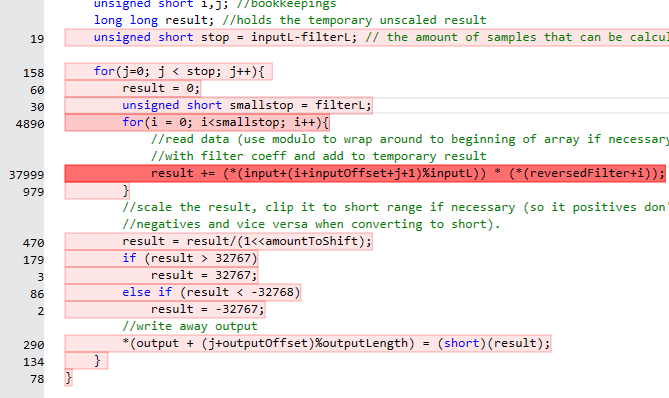
\includegraphics[width=\textwidth]{slow_convolve_cropped}
\caption{Unoptimized}
\end{subfigure}
\begin{subfigure}[c]{.7\textwidth}
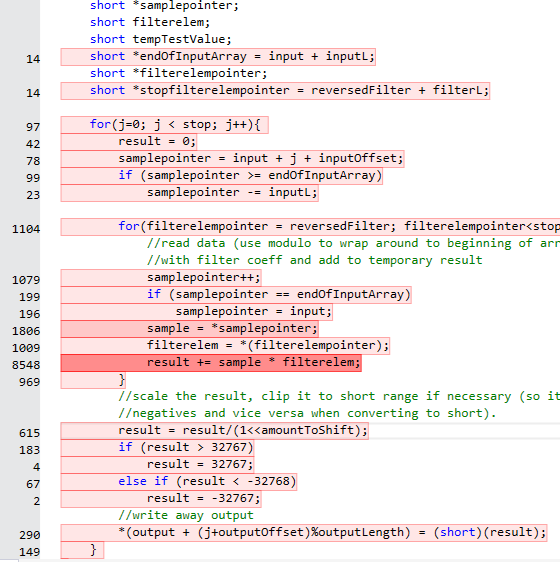
\includegraphics[width=\textwidth]{optimized_convolve_cropped}
\caption{Optimized}
\end{subfigure}
}
\caption{Details of unoptimized and optimized \texttt{convolve} functions}
\label{fig:convolvefunctions}
\end{figure}
\begin{minipage}{\textwidth}
The optimized version is derived from the unoptimized by:
\begin{itemize}
\item expanding the line of the inner loop to more substatements
\item using a pointer to the current filter element for the control of the inner \texttt{for}-loop instead of an additional counter. This saves variables and replaces additions by increments.
\item keeping and incrementing a pointer to the current data sample. This saves the complex calculation of the pointer. The expensive modulo operation of that calculation is reimplemented by two simple \texttt{if}-statements.
\end{itemize}
\end{minipage}

\section{Evaluation of the initial C implementation}
The MATLAB code is successfully translated to a C implementation. Both implementations produce the exact same output. Changes made to the MATLAB code to make its rounding mechanism the same as C's and vice versa are explained. Above text also illustrated why the C implementation is less flexible and works buffer per buffer. Next, it explained that bitwise operations were used in order to group useful bits. This is new in the C implementation: there is no equivalent in MATLAB. This is a preparation to communicate with an encryption algorithm, which will be provided by another group in the near future. The above text also handled about saving memory by using functions that work in-place, and about saving execution time. The latter was realized by profiling the code, and optimizing the critical inner loop of the \texttt{convolve} function. This enhanced execution time with approximately a factor 2. Previous text also explained how both the buffer per buffer execution order and the use of pointers made debugging harder, and the measure taken to facilitate this.

\section{Digital Signal Processor}
Next, the fully functional C implementation is ported to and optimized for a Digital Signal Processor. The DSP in question is the Texas Instruments TMS320C6748. 

\subsection{Optimization for DSP}
After already speeding up the code by a factor of about 2, running the application with an input file of 2986 samples resulted in 21.8M cycles: 7.300 cycles / sample. We will now discuss some of the changes that had the most influence on the cycle count. \\

The bottleneck was, as we suspected by analytical approach, convolve. This is because convolve contained the only nested loop, and worked with the biggest data types. The original convolve function was changed so that it could do both left and right channels in one call. The hypothesis was that this would give the compiler more freedom to use parallelism and that the decrease in overhead would also result in a small gain. Simulations showed a net gain of 8\% on the whole program.\\

Next, changing the result variables from a long long types to type int caused a gain of 49\% (!) on the whole program. This is a very large gain for a very simple optimization. The correctness of this change was tested with MATLAB, which showed no difference in the output at all since the 32-bit range was never exceeded. This changed moved the bottleneck away from convolve.\\

The new bottlenecks were quantize and dequantize. Again changing some variables to smaller types, combined with using restrict, lead to a gain of 42\% on the whole program. At this point, the assembly code showed a call to a divide function and this lead to a disqualification of the loop for software pipelining. Apart from this drawback, profiling also showed a large difference in inclusive and exclusive cycle counts for the quantize and dequantize functions. This indicates that most of the time was spent in the calls. Therefore, the code was rewritten to eliminate the calls. Division operations that expect a large quotient are now replaced by a binary search. Division operations that expect a small quotient are now replaced by a linear search. Both searches give the same output as the divisions. Figure \ref{fig:new_divisions} shows these changes. This saved 38.5\% of the cycles spent in these functions.\\

\begin{figure}
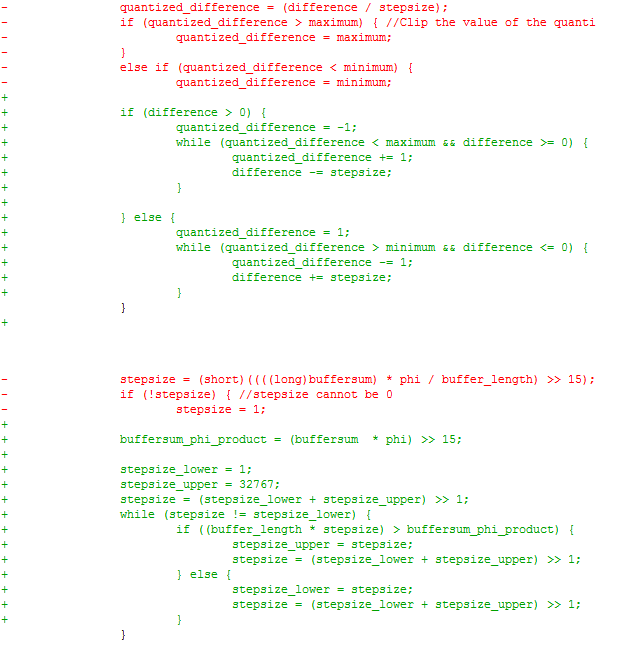
\includegraphics[width=\textwidth]{new_divisions}
\caption{Rewritten divisions in quantize and dequantize}
\label{fig:new_divisions}
\end{figure}
Improving these functions made convolve the bottleneck once again. Here, a division was written as \texttt{/(1<<amountToShift)}. This way was originally preferred over a simpler and faster \texttt{>>amountToShift} because it rounds towards zero instead of towards negative infinity, leading to a better PESQ score according to MATLAB simulations. Although at other points in the code the same type of division was optimized by the compiler, it was implemented as a call to a division function in convolve. Therefore another way to do this was necessary to eliminate the call. Exploiting the fact that it's a division by a power of two, the division is implemented as showed in figure \ref{fig:new_division_in_convolve}. The improvement sped up convolve by 46\%.\\

\begin{figure}
\makebox[\textwidth][c]{
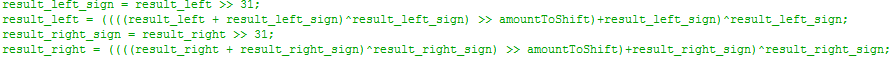
\includegraphics[width=1.4\textwidth]{new_division_in_convolve}
}
\caption{Rewritten division in convolve}
\label{fig:new_division_in_convolve}
\end{figure}
Finally, in convolve, combine and combineWithoutDelay the calls to a \texttt{reminder} function were eliminated. This gave a gain of 11\% on convolve and 68\% on combine. Together with rewriting the divisions, this gave a reduction of 39\% for the total application.\\

As a last change, we changed the quantization and dequantization functions to work on the left and right channel together. This gave a reduction of 11\%.\\
These major optimizations can be found in table \ref{table:optimizations}. Please note that they are not the only optimizations we tried: in fact, we tried every optimization that was suggested in the powerpoint. This includes:
\begin{itemize}
\item Hardcoding filter coefficients, instead of fetching them from data. Hoping this would lead to a speed up because less data accesses are necessary and because the basic block is larger, leading to more parallelism possibilities. However, this did not gain us as much as we'd expect, so we reverted this to have more flexibility.
\item Pragmas: MUST\_ITERATE, UNROLL. We used these wherever possible. In some cases, they did deliver a certain gain, in other cases they didn't.
\item Pragma: DATA\_ALIGN. We tried this, together with the intrinsic \_nassert, but this didn't result in any improvement. We guess that this is because the compiler had already optimized this data.
\item Intrinsics: We tried many intrinsics, but the only one that we found to be useful is '\_abs'. Sometimes using SIMD instructions for parallelism did not help, because it replaced parallelism by using two cores created by the compiler.
\item 'Near' and 'const' variable keywords: These keywords did not give us any or much gain, and we reverted this optimization for cleanliness.
\item 'Restrict' variable keyword: This keyword was used wherever possible, and often gave improvements.
\item Function inlining: we tried inlining the whole analysis and synthesis files, but at that point the amount of cycles saved the gain was not big enough to make a noticeable difference. Thus we reverted this for cleanliness. After other speed-ups, it might now be non-negligible, but together with the code of the crypto group, there is not enough text space available to do so.
\end{itemize}

After all optimizations, the program used 3.2M cycles for 2986 samples, equalling 1072 cycles/sample. This number has to be interpreted with some context:
\begin{itemize}
\item The cycle count includes reading the .wav-file, doing all the processing, and writing the .wav-file, whereas other groups may only count (a part of) the processing. Actually, the writing of the .wav-file, a function that has been provided with the assigment, is the new bottleneck.
\item The audio file that is used as input has 2986 samples, but is mono instead of stereo: it has only one channel. This means that every sample will be doubled, effectively resulting in 5972 samples. We count one left/right combination as one sample, while we heard some other groups count this as two. In their way of thinking, we come to 536 cycles per sample.
\end{itemize}
All this results in a total speed-up of 85\% or a factor 6.8 for the DSP part, and times 13.6 in combination with the C part.\\

A last optimization that we'd like to mention is what we call 'cheatMono': We noticed that a lot of the input signals were mono instead of stereo, and thus a lot of computational power was being wasted. As a proof of concept, we wrote new functions 'quantizeMono' and 'dequantizeMono' which operated on the left channel and copied the results to the right channel. In the case of stereo input, the only change is one if-statement that has to be evaluated for every buffer of 40 input samples. This optimization results in a reduction of 16\% of the cycles of the whole program in case of mono input. The downside is that 2\% more of the available space is used as code text. Since this is not a part of the original project description, we have not included this gain in our final cycle count, but we have included this functionality in our project. 

\begin{table}
\makebox[\linewidth][c]{
\begin{tabular}{|p{2cm}|p{3cm}|p{3cm}|p{2cm}|p{2cm}|p{1cm}|}
\hline 
• & Major Optimization & Functions Effected & Cycles Before & Cycles After & Change (in \%) \\ 
\hline 
Base Code & • & • & 21.8M & • & • \\ 
\hline 
Session 1 & Hardcoded filter coefficients & Convolve (reverted) & 21.8M & 21.7M (reverted) & .05 (reverted)\\ 
\hline 
Session 2 & Combine convolve left and right & Convolve & 21.8M & 20.1M & 8 \\ 
\hline 
Session 3 & Long long to int & Convolve & 20.1M & 10.2M & 49 \\ 
\hline 
Session 4 & Restrict variables (global), change variable types & (de)quantize & 10.2M & 5.9M & 42 \\ 
\hline 
Session 5 & Merge with crypto, try to get DSP working & & 5.9M & 5.9M & \\
\hline
Session 6 & Wrote divisions as binary or linear search & (de)quantize & 5.9M & 3.6M & 39 \\
\hline
& Wrote divisions as shift (with rounding to zero) & Convolve & & & \\
\hline
& Remove modulo in output index & Convolve & & & \\
\hline
& Remove modulo in indices & Combine, combineWithoutDelay & & & \\
\hline
Extra session & Change some unrolls, must\_iterates & Global & 3.6M & 3.2M & 11 \\
\hline
& Combine left and right (de)quantize & (de)quantize & & & \\
\hline
\end{tabular} 
}
\caption{Table with major optimizations}
\label{table:optimizations}
\end{table}

\section{Application description}
The structure of the C/DSP code is the same as the MATLAB structure. The .c-files are largely the same as the MATLAB files. Some small extra functions were made to transfer data or sum arrays. All functions are well documented, so please refer to this documentation for further explanation of their function and use. Another difference is that for the DSP version, we use \texttt{quantizeTogether} and \texttt{dequantizeTogether} instead of \texttt{quantize} and \texttt{dequantize}, because this is more efficient.

The application is executed by running main.c. Enabling the cryptography part from another group and enabling cheating mono input signals is done by defining 'CRYPTO' and 'cheatMono' respectively, as can be seen in globals.h. The input and output .wav-file can also be specified in globals.h.

\section{Porting and integration}
Porting the project from Linux/Windows to the CCS simulator was well explained and we simply followed the presentation. \\

The integration with the crypto group was smooth as well. We decided on a crypto buffer of 600 chars long. Every input buffer that we read consists of 40 samples (shorts). We discard the highest band, or 10 samples per input buffer. The remaining 30 shorts are compressed into 15 bytes after they have been quantized. This fits perfectly, and no bits are wasted. In total, 40 input buffers of 40 samples fit into one crypto buffer after processing. This causes a total delay of: $40*40/2/8000 = 100ms$. The factor 2 comes from the fact that input is stereo and thus has two channels, each operating at 8kHz. \\
The only issue that we faced when integrating with the crypto group, is that the DSP has limited memory. This was never a real problem, but limited for example the inlining that could be done. \\
Switching from the simulator to the real DSP did cause us some headaches. First, we had a problem where we apparently forgot to initialize a variable. This was resolved, obviously, by initializing it. Then the DSP still wouldn't produce the correct output, even though we didn't know why. We spent almost an entire session on this problem, only to find out that the DSP we were given, was malconfigured: some of the switches on top were not set properly. After correcting the switches, the DSP worked fine, proving our code was correct. \\
We then tried using it real-time, but this didn't work. We spent most of our remaining time on this issue, but sadly could not get it to work.

\section{Lessons learnt}
These are three things that we will remember from this project:
\begin{itemize}
\item Initializing variables is important and can easily be forgotten for some variables.
\item Simply reducing variable types can result in quick but impactful optimizations.
\item Always check if the hardware (DSP) that you get is configured correctly.
\item When optimizing code for the DSP, the effects of changes are not always predictable.
\end{itemize}

\section{Conclusions}
This was the final report for the P\&D assignment on creating a speech codec. A speech codec has been succesfully created and works on the DSP simulator, but sadly not in real-time. \\

The paper first explained the key concepts of the codec: QMF subband splitting and adaptive differential quantization. Then, the MATLAB implementation was thoroughly explained. The paper explained that during optimizing, a high average PESQ score was targetted and that optimizing was done by hand, changing the values in greedy like approach. The achieved PESQ scores ranged from 3.00 to 3.54, depending on the file. This indicates decent performance.\\

Next, the transition to C code was covered. The execution order and loss of flexibility were identified as differences between the MATLAB and C implementations. The paper explained the use of the new compress and decompress functions which pack and unpack the usefull bits, as preparation to integrate with an encryption group. It also addressed performance enhancements that were made before porting to a DSP. These sped up the code by a factor of 2. \\

Finally, there was a transition from C to the DSP simulator and eventually to the DSP itself. The actual porting onto the simulator and the integration with the crypto group did not raise problems. Running it on the actual DSP did cause some headaches though, caused by not proper initializing all variables and a wrongly configured DSP. The paper discussed the optimizations that were made to make the code more efficient, leading to another speed-up factor of 6.8. The main optimizations leading to this factor are smaller variable types and elimination of calls to division and reminder functions. More classical 'tricks' to improve performance, like pragmas and intrinsics, did not seem to help as much on our code.\\

Finally, this paper ends with the lessons that we learned and a personal course evaluation. \\

If one were to work further on this project, a good thing to do would be to implement more intrinsics. When used correctly, these specialised lowest-level instructions are capable or speeding up the system quite a bit. However, for this to be possible, the high level structure of the code may have to be changed.

\section{Course evaluation}
Overall, we enjoyed working on this project. The workload is okay and the topic is interesting. The supervision was good for the C and DSP part, but lacked for the MATLAB part.
We think that the MATLAB code could be provided to the students, since we already know how to program in MATLAB and it's more of a time sink, whereas optimizing for a DSP is new and exciting work.
\end{document}
